\chapter{Introduction}


% Description of large-scale structure in our universe
%  - What has been observed?
%  - What has been simulated?

\begin{figure}
    \includegraphics[width=0.65\textwidth]{Images/Intro/sdss}
    \caption[SDSS galaxy map]{A slice through the SDSS galaxy distribution; each 
    point on this plot is a galaxy.  Large sky surveys such as SDSS have 
    revealed a non-uniform distribution of galaxies throughout the universe.  
    Dubbed the cosmic web, galaxies clump together in clusters and along 
    filaments, leaving giant gaps between them (similar to a sponge).}
    \label{fig:SDSS_map}
\end{figure}

\begin{figure}
%    \includegraphics[width=0.9\textwidth]{Images/Intro/Millenium_simulation}
    \caption[Dark matter simulation]{Snapshots of a portion of the Millenium 
    Simulation showing the dark matter distribution at different points in time 
    from 0.21 Gyr after the Big Bang to the present.  Small perturbations in the 
    initial distribution of dark matter are amplified as the universe expands.  
    Gravity causes the slightly overdense regions to contract while 
    simultaneously causing the underdense regions to expand.}
    \label{fig:DMsim}
\end{figure}

Large sky surveys \citep[such as the Sloan Digital Sky Survey --- 
SDSS][]{York00} have revealed a non-uniform distribution of galaxies throughout 
the universe.  Taking on a shape similar to that of a three-dimensional cosmic 
web \citep{Bond96} or a sponge, galaxies clump together in clusters and along 
filaments, leaving void regions between them.  Evidence of this distribution can 
be seen in Fig. \ref{fig:SDSS_map} for galaxies in the SDSS Data Release 7 
\citep[SDSS DR7][]{Abazajian09}.  Based on these observations, dark matter 
simulations have been constructed which successfully reproduce the same 
large-scale structure.  If we start with a mostly uniform distribution of dark 
matter at the Big Bang, Fig. \ref{fig:DMsim} outlines the evolution of that dark 
matter up to present day.  These snapshots from the Millenium Simulation project 
\citep{Springel05} show that small perturbations in the initial distribution of 
dark matter are amplified as the universe expands.  Gravity causes the slightly 
overdense regions to collapse while simultaneously causing the underdense 
regions to expand.  Due to dark matter's strong gravitational interaction, we 
believe that the baryonic mattter (that which interacts electromagnetically) 
will trace the dark matter distribution, resulting in the galaxy distribution we 
observe today.


% Void galaxies
\begin{figure}
%    \includegraphics[width=0.9\textwidth]{Images/Intro/void_slice}
    \caption[Sky map highlighting voids and void galaxies]{A 10 \hMpc slice of 
    SDSS DR7 \citep[Fig. 1]{Moorman14} with void regions highlighted in blue 
    circles.  Void galaxies are shown as red points while wall galaxies are 
    black.  Existing in the cosmological voids (space between the galactic 
    filaments), void galaxies are though to demonstrate the fundamental 
    characteristics of galactic evolution.}
\end{figure}

The galaxies within the underdense void environments are named ``void 
galaxies.''  Existing in the cosmological voids, void galaxies are thought to 
demonstrate the fundamental characteristics of galactic evolution.  Cosmic voids 
are an important environment for studying galaxy formation \citep[see][for a 
review]{vandeWeygaert11}.  Gravitational clustering proceeds as if in a very low 
density universe, where the amassment of gravitationally bound dark matter halos 
ends relatively early and there is little subsequent interaction between the 
galaxies due to the lower density and the faster local Hubble expansion.  
Therefore, $\Lambda$CDM cosmology predicts that galaxies formed in voids should 
have lower mass and be retarded in their star formation when compared to those 
in denser regions \cite[e.g.,][]{Gottlober03,Goldberg05,Cen11}.  
\cite{Goldberg04} show that a void region that is only 10\% of the mean density 
of the universe with $\Omega_{matter} = 0.3$, $h = 0.7$ dynamically evolves as 
if $\Omega_{matter} = 0.02$, $\Omega_\Lambda = 0.48$, and $h = 0.84$.  
Additionally, hydrodynamical cosmological simulations by \cite{Cen11} show that 
the gas in voids remains below the critical entropy threshold, allowing void 
galaxies to continue to form stars.  Void galaxies evolve in a relatively 
pristine environment where interactions are rare and star formation proceeds up 
to the present epoch because void galaxies are able to retain their gas.  This 
contrasts the denser environments, where the chemical composition and evolution 
of galaxies are drastically altered due to mergers and tidal stripping and/or 
ram-pressure stripping.

% What do we already know about the environmental influence?



% Dwarf galaxies

\begin{figure}
    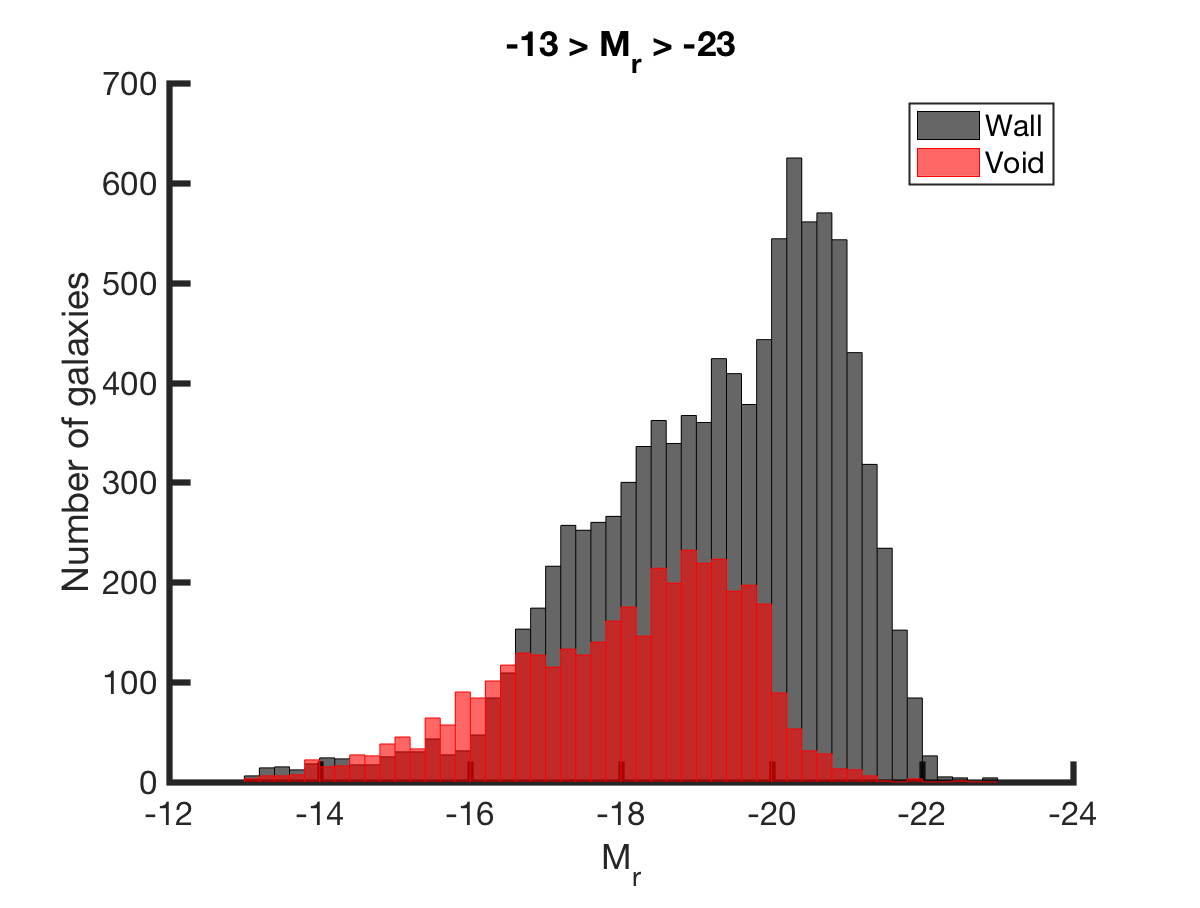
\includegraphics[width=0.65\textwidth]{Images/Intro/1sig_13-23_SDSS_Mr_hist_count_fill}
    \caption[Absolute magnitude distribution of galaxies in SDSS DR7]{Absolute 
    magnitude ($M_r$) distribution of galaxies in SDSS DR7, separated into void 
    and wall environments.  Dwarf galaxies are defined as galaxies with absolute 
    magnitudes fainter than -17 ($M_r > -17$).  For reference, the Milky Way has 
    an absolute magnitude $M_r \approx -20$.}
\end{figure}



% Galaxy structure




% Metallicity
%  - How are elements synthesized in stars?
%  - What does the light look like when it reaches us?  When we look at an emission spectrum, what are we studying?
%  - What are forbidden transitions and why are they important?
%  - How do we get the temperature from the emission line ratio?  (Summary - refer to appendix for more details)
%  - What is the metallicity?  O/H - Why oxygen?  and once we estimate the abundances of each ion, we add them together to get the total abundance for that element

\begin{figure}
    \includegraphics[width=0.9\textwidth]{Images/Intro/Kirchoff}
    \caption[Kirchoff's laws of spectroscopy]{Three different viewpoints of the 
    light emitted from a star and/or a cool cloud of gas, representing 
    Kirchoff's laws of spectroscopy.  A star emits light across all wavelengths, 
    so the resulting spectrum is known as a continuous spectrum.  Star's light 
    that has passed through a cloud of cool gas before being observed is an 
    absorption spectrum, where the elements in the cloud have absorbed some of 
    the light at specific wavelengths (corresponding to the particular elements 
    present in the gas).  If observed off the line-of-sight of the star, the 
    light emitted from the cloud of cooler gas is named an emission spectrum, 
    where the gas is re-radiating the light it absorbed from the star.}
\end{figure}

\begin{figure}
%    \includegraphics[width=0.9\textwidth]{Images/Intro/spectrum}
    \caption[Sample (void) dwarf galaxy spectrum]{Example SDSS DR7 spectrum --- 
    this is a void dwarf galaxy whose gas-phase chemical abundances are slightly 
    above average.  The [\ion{O}{3}] $\lambda$4363 auroral line is circled in 
    red, while the [\ion{O}{3}] $\lambda \lambda$4959,5007 doublet is circled in 
    yellow.}
\end{figure}


% Outline of Thesis
% Pose the problem - how does the large-scale environment affect galaxy evolution?
We want to understand how dark matter affects the evolution of a galaxy, and 
what influence it has on a galaxy's star formation.  To do this, we compare the 
properties of galaxies living in voids with galaxies in denser regions in an 
effort to understand how the properties of the gas and the history of star 
formation in a galaxy depend on the environment.  We then try to infer what 
these results tell us about the dark matter structure and history of the galaxy.